\documentclass{article}

\usepackage{amsthm}
\usepackage{amsfonts}
\usepackage{amsmath}
\usepackage{amssymb}
\usepackage{fullpage}
\usepackage[usenames]{color}
\usepackage{hyperref}
  \hypersetup{
    colorlinks = true,
    urlcolor = blue,       % color of external links using \href
    linkcolor= blue,       % color of internal links
    citecolor= blue,       % color of links to bibliography
    filecolor= blue,        % color of file links
    }

\usepackage{listings}
\usepackage{graphicx}
\graphicspath{ {./Report Images/} }

\definecolor{dkgreen}{rgb}{0,0.6,0}
\definecolor{gray}{rgb}{0.5,0.5,0.5}
\definecolor{mauve}{rgb}{0.58,0,0.82}

\lstset{frame=tb,
  language=haskell,
  aboveskip=3mm,
  belowskip=3mm,
  showstringspaces=false,
  columns=flexible,
  basicstyle={\small\ttfamily},
  numbers=none,
  numberstyle=\tiny\color{gray},
  keywordstyle=\color{blue},
  commentstyle=\color{dkgreen},
  stringstyle=\color{mauve},
  breaklines=true,
  breakatwhitespace=true,
  tabsize=3
}

\theoremstyle{theorem}
   \newtheorem{theorem}{Theorem}[section]
   \newtheorem{corollary}[theorem]{Corollary}
   \newtheorem{lemma}[theorem]{Lemma}
   \newtheorem{proposition}[theorem]{Proposition}
\theoremstyle{definition}
   \newtheorem{definition}[theorem]{Definition}
   \newtheorem{example}[theorem]{Example}
\theoremstyle{remark}
  \newtheorem{remark}[theorem]{Remark}


\title{CPSC-354 Report}
\author{Marc Domingo  \\ Chapman University}

\date{\today}

\begin{document}

\maketitle
\section{Introduction}\label{introduction}
\subsection{Week 1}
\hspace{10mm} During the first week of Programming Languages, the class lectures went over the concept of \textit{Imperative vs Functional Programming} and \textit{Recursive Programming} in addition to a brief introduction to the programming language \textbf{Haskell}.
\subsection{Week 2}
\hspace{10mm} During the second week of Programming Languages, the class lectures went more into depth regarding techniques in how to use \textbf{Recursion} to solve problems, as well as introduced the concept of creating an \textit{Interpreter} in Haskell.
\subsection{Week 3} During the third week of Programming Languages, the class lectures went over the concept of Context and Parse Trees in relation to programming a calculator interpreter.
\subsection{Week 4} During the fourth week of Programming Languages, the lectures covered the concept of Lambda Calculus, specifically about its syntax and how to parse Lambda equations.
\section{Homework}\label{homework}
\subsection{Week 1}

C++ Code for Greatest Common Denominator:
\begin{lstlisting}
#include <iostream>
using namespace std;

int gcd(int a, int b)
{
    if (a == 0)
    {
        return b;
    }

    if (b == 0)
    {
        return a;
    }

    if (a == b)
    {
        return a;
    }

    if (a > b)
    {
        return gcd((a - b), b);
    }

    if (b > a)
    {
        return gcd(a, (b - a));
    }
}

int main() {
    // Write C++ code here
    cout << "GCD of 9 and 33 is : " << gcd(9, 33);
    return 0;
}
\end{lstlisting}

    The function for calculating the Greatest Common Divisor (GCD) functions by first taking two integers as inputs, represented by \textbf{a} and \textbf{b}. In the case of inputs like gcd(9, 33), 9 and 33 are considered to be \textbf{a} and \textbf{b} in the gcd function respectively. The function first checks to see if either integer is \textit{0}, and in the case of either integer being zero, returns the other integer entered in the function as the gcd. If neither number is zero, the function checks to see if both integers are \textbf{equal to each other}. In the case that both integers are equal, the function returns the first integer as the gcd. If neither of the previous cases are met, the function then compares integer \textbf{a} and \textbf{b}. If integer \textbf{a} is larger, the function recursively calls itself, and \textit{integer a is replaced with (a - b)}. If integer \textbf{b} is larger, the function recursively calls itself, and \textit{integer b is replaced with (b - a).} The function \textit{continues making recursive calls} with modified numbers until a case where gcd is found.

\subsection{Week 2}
\begin{lstlisting}
len [] = 0
len (x:xs) = 1 + len xs

select_evens [] = []
select_evens [a] = []
select_evens (x:y:list) = y:(select_evens list)

select_odds [] = []
select_odds [a] = [a]
select_odds (x:y:list) = x:(select_odds list)

member _ [] = False
member n (x:xs)
  | x == n = True
  | otherwise = member n xs

append [] list_original = list_original
append (x:list_add) list_original = x:(append list_add list_original)

revert [] = []
revert (item:xs) = append (revert xs) [item]

less_equal [] [] = True
less_equal (x:list_one) (y:list_two) = if x <= y
									    then less_equal list_one list_two
									    else False
\end{lstlisting}
In the case of \textbf{select\textunderscore evens ["a","b","c","d","e"]}:
\begin{lstlisting}
select_evens ["a","b","c","d","e"] =
      "b":(select_evens ["c","d","e"]) =
      "b":"d":(select_evens ["e"]) =
      "b":"d":[] =
      ["b","d"]
\end{lstlisting}
In the case of \textbf{select\textunderscore odds ["a","b","c","d","e"]}:
\begin{lstlisting}
select_odds ["a","b","c","d","e"] =
      "a":(select_odds ["c","d","e"]) =
      "a":"c":(select_odds ["e"]) =
      "a":"c":["e"] =
      ["a","c","e"]
\end{lstlisting}
In the case of \textbf{member 2 [5,2,6]}:
\begin{lstlisting}
member 2 [5,2,6] =
        member 2 [2,6] =          5 != 2
        True                      2 == 2
\end{lstlisting}
In the case of \textbf{member 3 [5,2,6]}
\begin{lstlisting}
member 3 [5,2,6] =
      member 3 [2,6] =          5 != 3
      member 3 [6] =            2 != 3
      member 3 [] =             6 != 3
      False
\end{lstlisting}
In the case of \textbf{append [1,2] [3,4,5]}:
\begin{lstlisting}
append [1,2] [3,4,5] =
      1:(append [2] [3,4,5]) =
      1:(2:(append [] [3,4,5])) =
      1:(2:([3:4:5])) =
      [1,2,3,4,5]
\end{lstlisting}
In the case of \textbf{revert [1,2,3]}:
\begin{lstlisting}
revert [1,2,3] =
      append (revert [2,3]) [1] =
      append (append (revert [3]) [2]) [1] =
      append (append (append (revert []) [3]) [2]) [1] =
      append (append (append [] [3]) [2]) [1] =
      append (append ([3]) [2]) [1] =
      append (3:(append [] ([2]))) [1] =
      append (3:([2]) [1] =
      append [3,2] [1] =
      3:(append [2] [1]) =
      3:(2:(append [] [1])) =
      3:(2:([1])) =
      [3,2,1]
\end{lstlisting}
In the case of \textbf{less\textunderscore equal [1,2,3] [2,3,4]}:
\begin{lstlisting}
less_equal [1,2,3] [2,3,4] =
      less_equal [2,3] [3,4] =          1 <= 2
      less_equal [3] [4] =              2 <= 3
      less_equal [] [] =                3 <= 4
      True
\end{lstlisting}
In the case of \textbf{less\textunderscore equal [1,2,3] [2,3,2]}:
\begin{lstlisting}
less_equal [1,2,3] [2,3,2] =
      less_equal [2,3] [3,2] =          1 <= 2
      less_equal [3] [2] =              2 <= 3
      False                             3 > 2
\end{lstlisting}

\subsection{Week 3}
\begin{lstlisting}
hanoi 5 0 2
    hanoi 4 0 1
        hanoi 3 0 2
            hanoi 2 0 1
                hanoi 1 0 2 = move 0 2
                move 0 1
                hanoi 1 2 1 = move 2 1
            move 0 2
            hanoi 2 1 2
                hanoi 1 1 0 = move 1 0
                move 1 2
                hanoi 1 0 2 = move 0 2
        move 0 1
        hanoi 3 2 1
            hanoi 2 2 0
                hanoi 1 2 1 = move 2 1
                move 2 0
                hanoi 1 1 0 = move 1 0
            move 2 1
            hanoi 2 0 1
                hanoi 1 0 2 = move 0 2
                move 0 1
                hanoi 1 2 1 = move 2 1
    move 0 2
    hanoi 4 1 2
        hanoi 3 1 0
            hanoi 2 1 2
                hanoi 1 1 0 = move 1 0
                move 1 2
                hanoi 1 0 2 = move 0 2
            move 1 0
            hanoi 2 2 0
                hanoi 1 2 1 = move 2 1
                move 2 0
                hanoi 1 1 0 = move 1 0
        move 1 2
        hanoi 3 0 2
            hanoi 2 0 1
                hanoi 1 0 2 = move 0 2
                move 0 1
                hanoi 1 2 1 = move 2 1
            move 0 2
            hanoi 2 1 2
                hanoi 1 1 0 = move 1 0
                move 1 2
                hanoi 1 0 2 = move 0 2
\end{lstlisting}
Movement solution for Towers of Hanoi with n Disks = 5:
\begin{lstlisting}
0->2
0->1
2->1
0->2
1->0
1->2
0->2
0->1
2->1
2->0
1->0
2->1
0->2
0->1
2->1
0->2
1->0
1->2
0->2
1->0
2->1
2->0
1->0
1->2
0->2
0->1
2->1
0->2
1->0
1->2
0->2
\end{lstlisting}
Within the computation for the Towers of Hanoi with \textit{n Disks = 5}, the word "Hanoi" appears a total of \textbf{31 times}. This can be expressed with the following equation:
$ Hanoi = 2^N - 1$, where \textit{N} is the number of disks from the initial tower.

\subsection{Week 4}
The Abstract Syntax Tree of $2 + 1$ is:

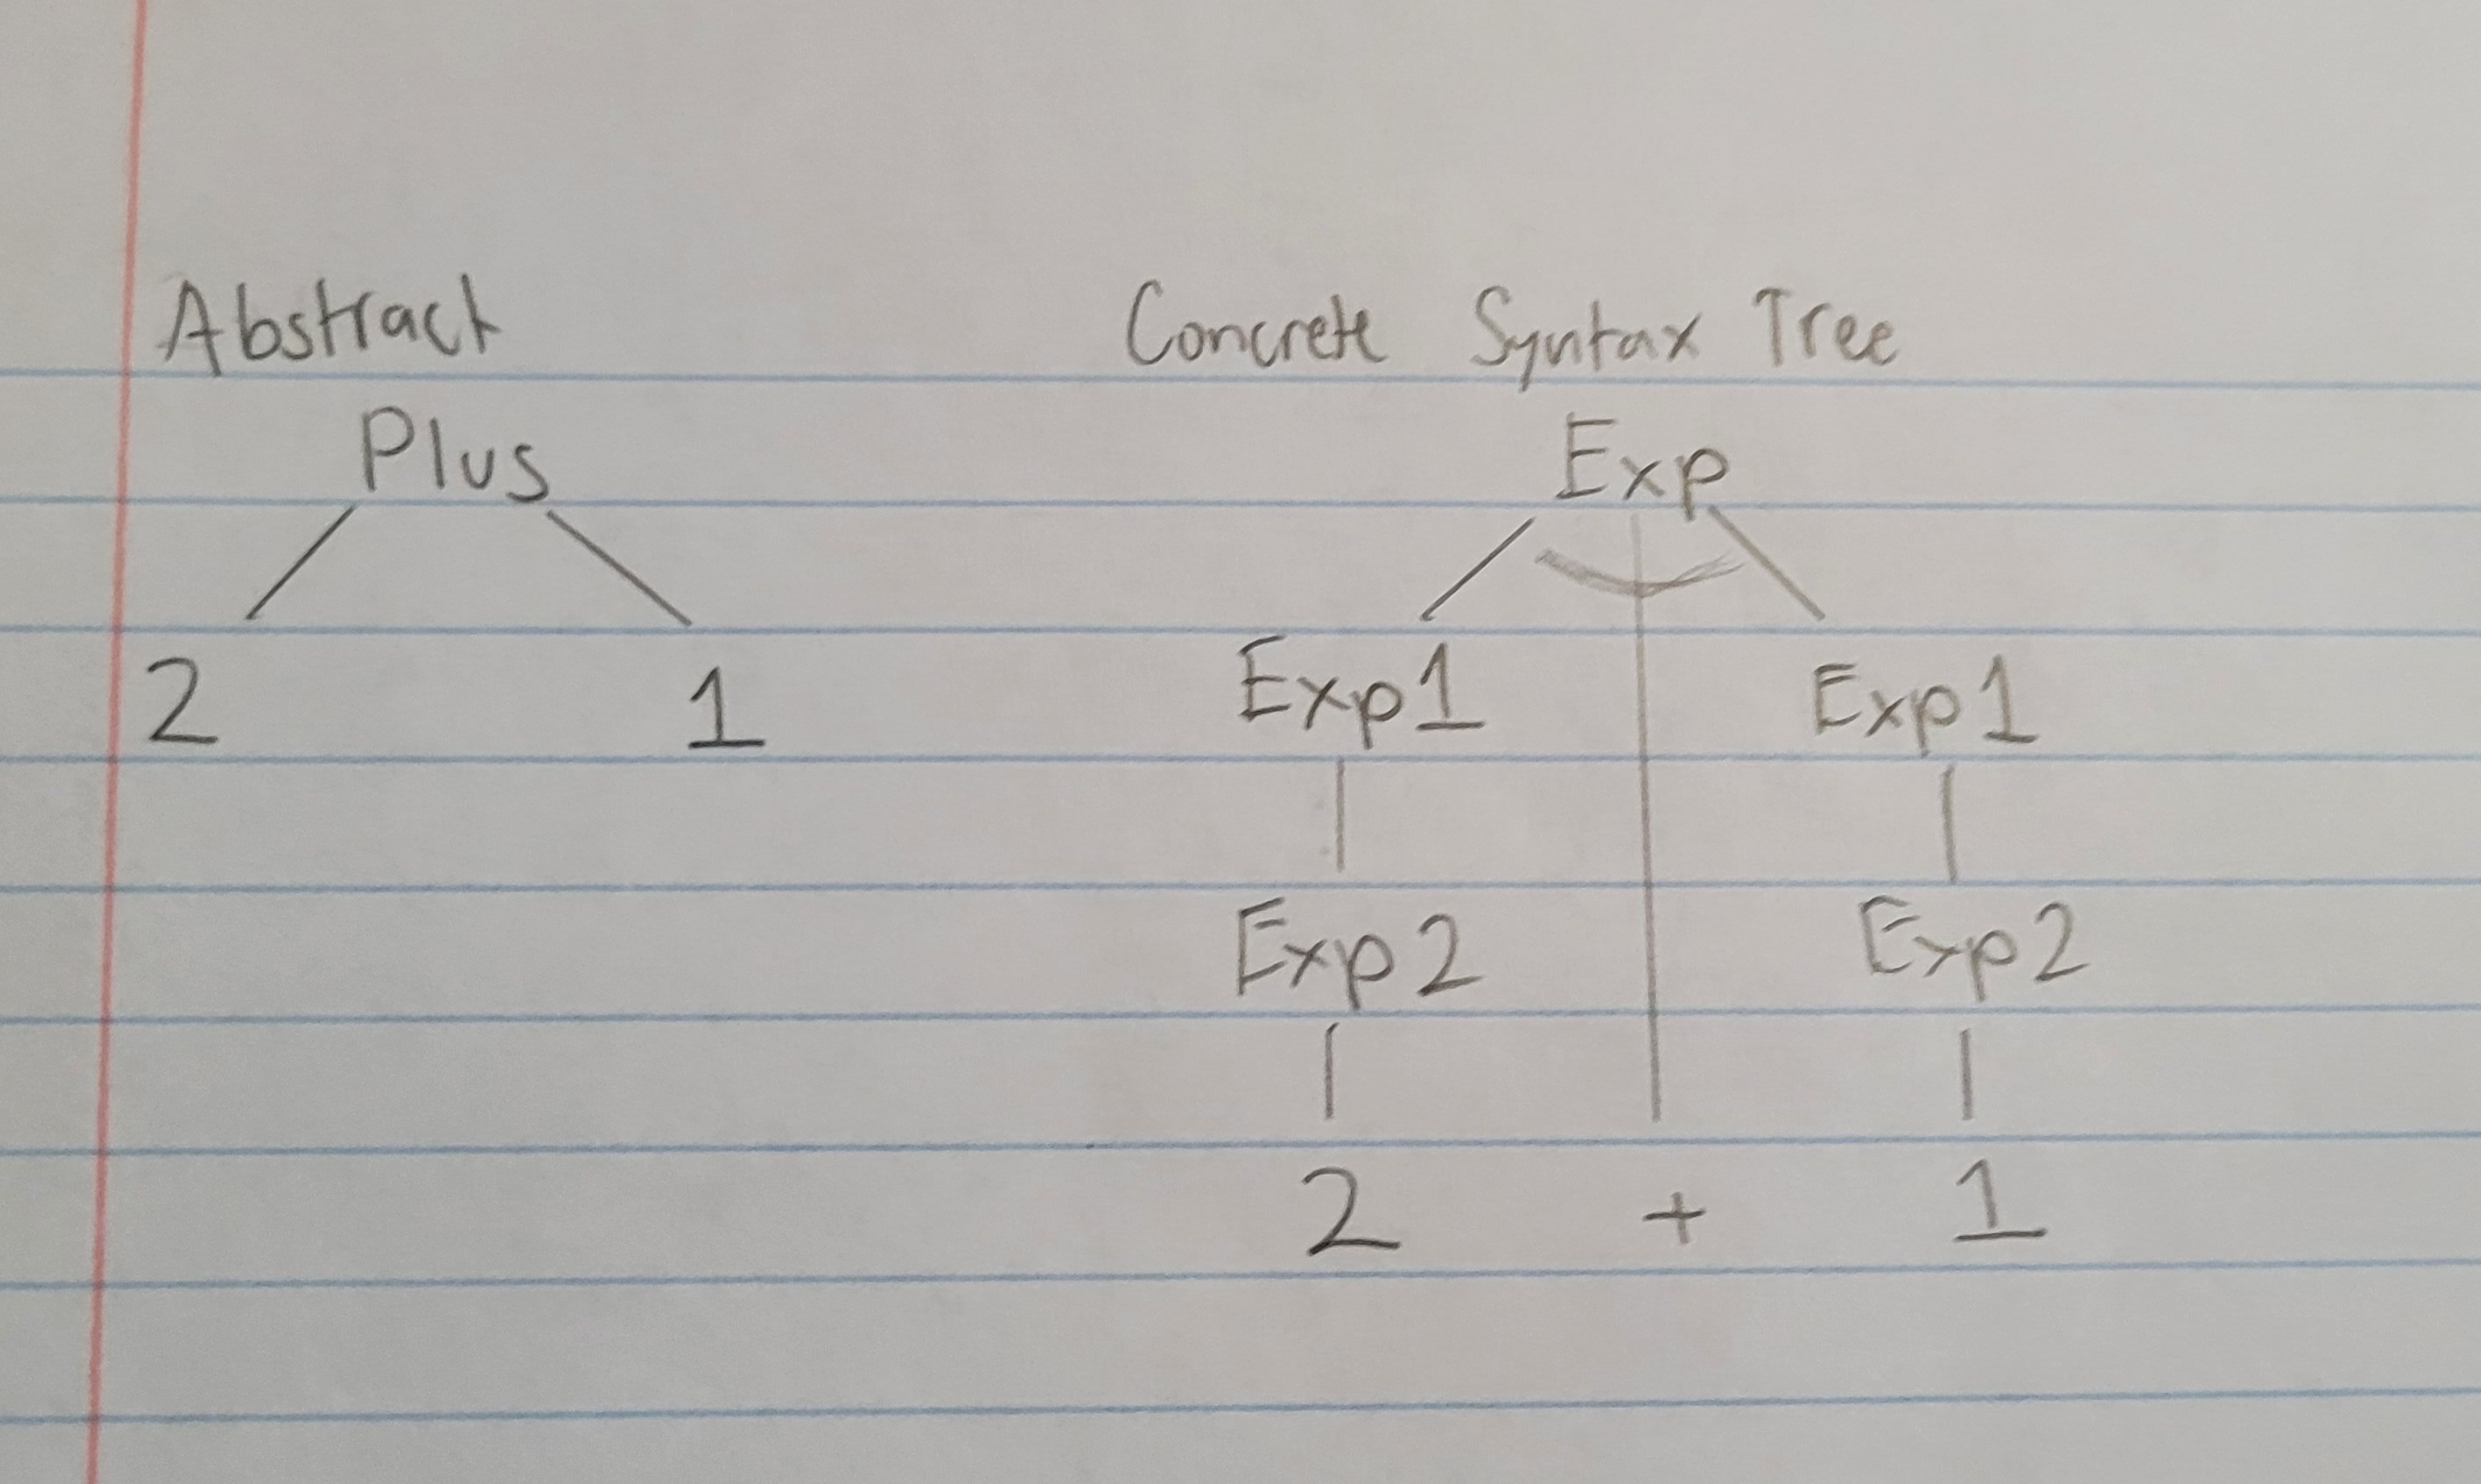
\includegraphics[width=15cm, height=8cm]{Report Images/week4_1.jpg}
\begin{lstlisting}
Plus (Num 2) (Num 1)
\end{lstlisting}


The Abstract Syntax Tree of $1 + 2 * 3$ is:

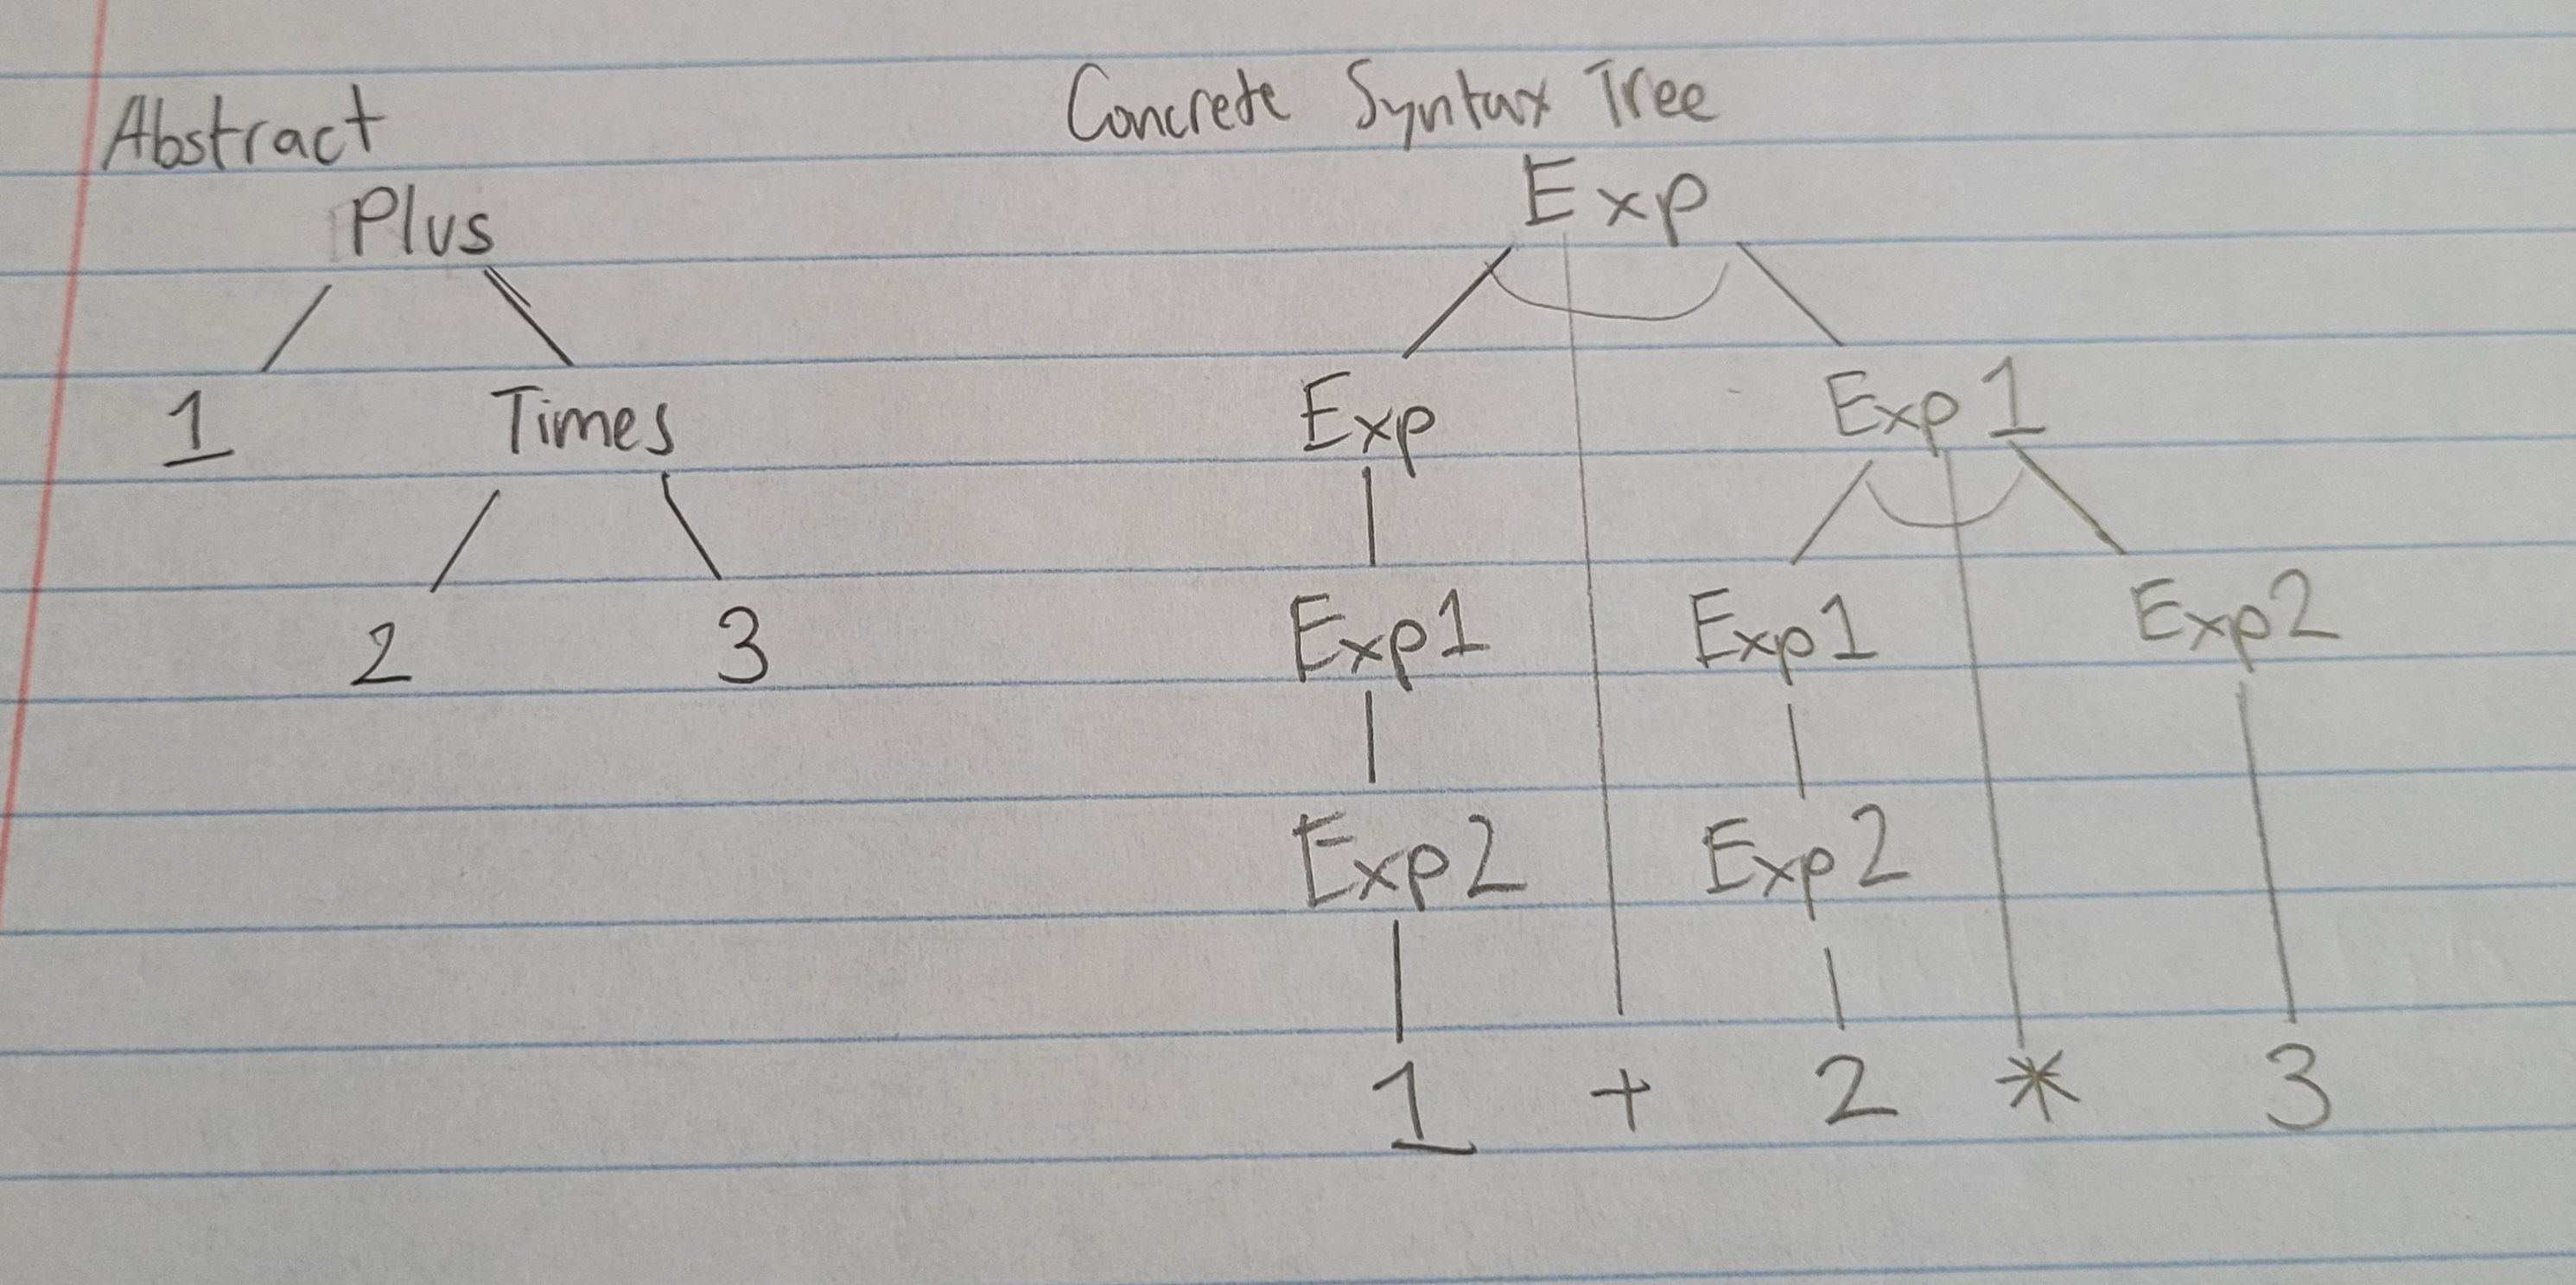
\includegraphics[width=15cm, height=8cm]{Report Images/week4_2.jpg}
\begin{lstlisting}
Plus (Num 1) (Times (Num 2) (Num 3))
\end{lstlisting}

The Abstract Syntax Tree of $1 + (2 * 3)$ is:

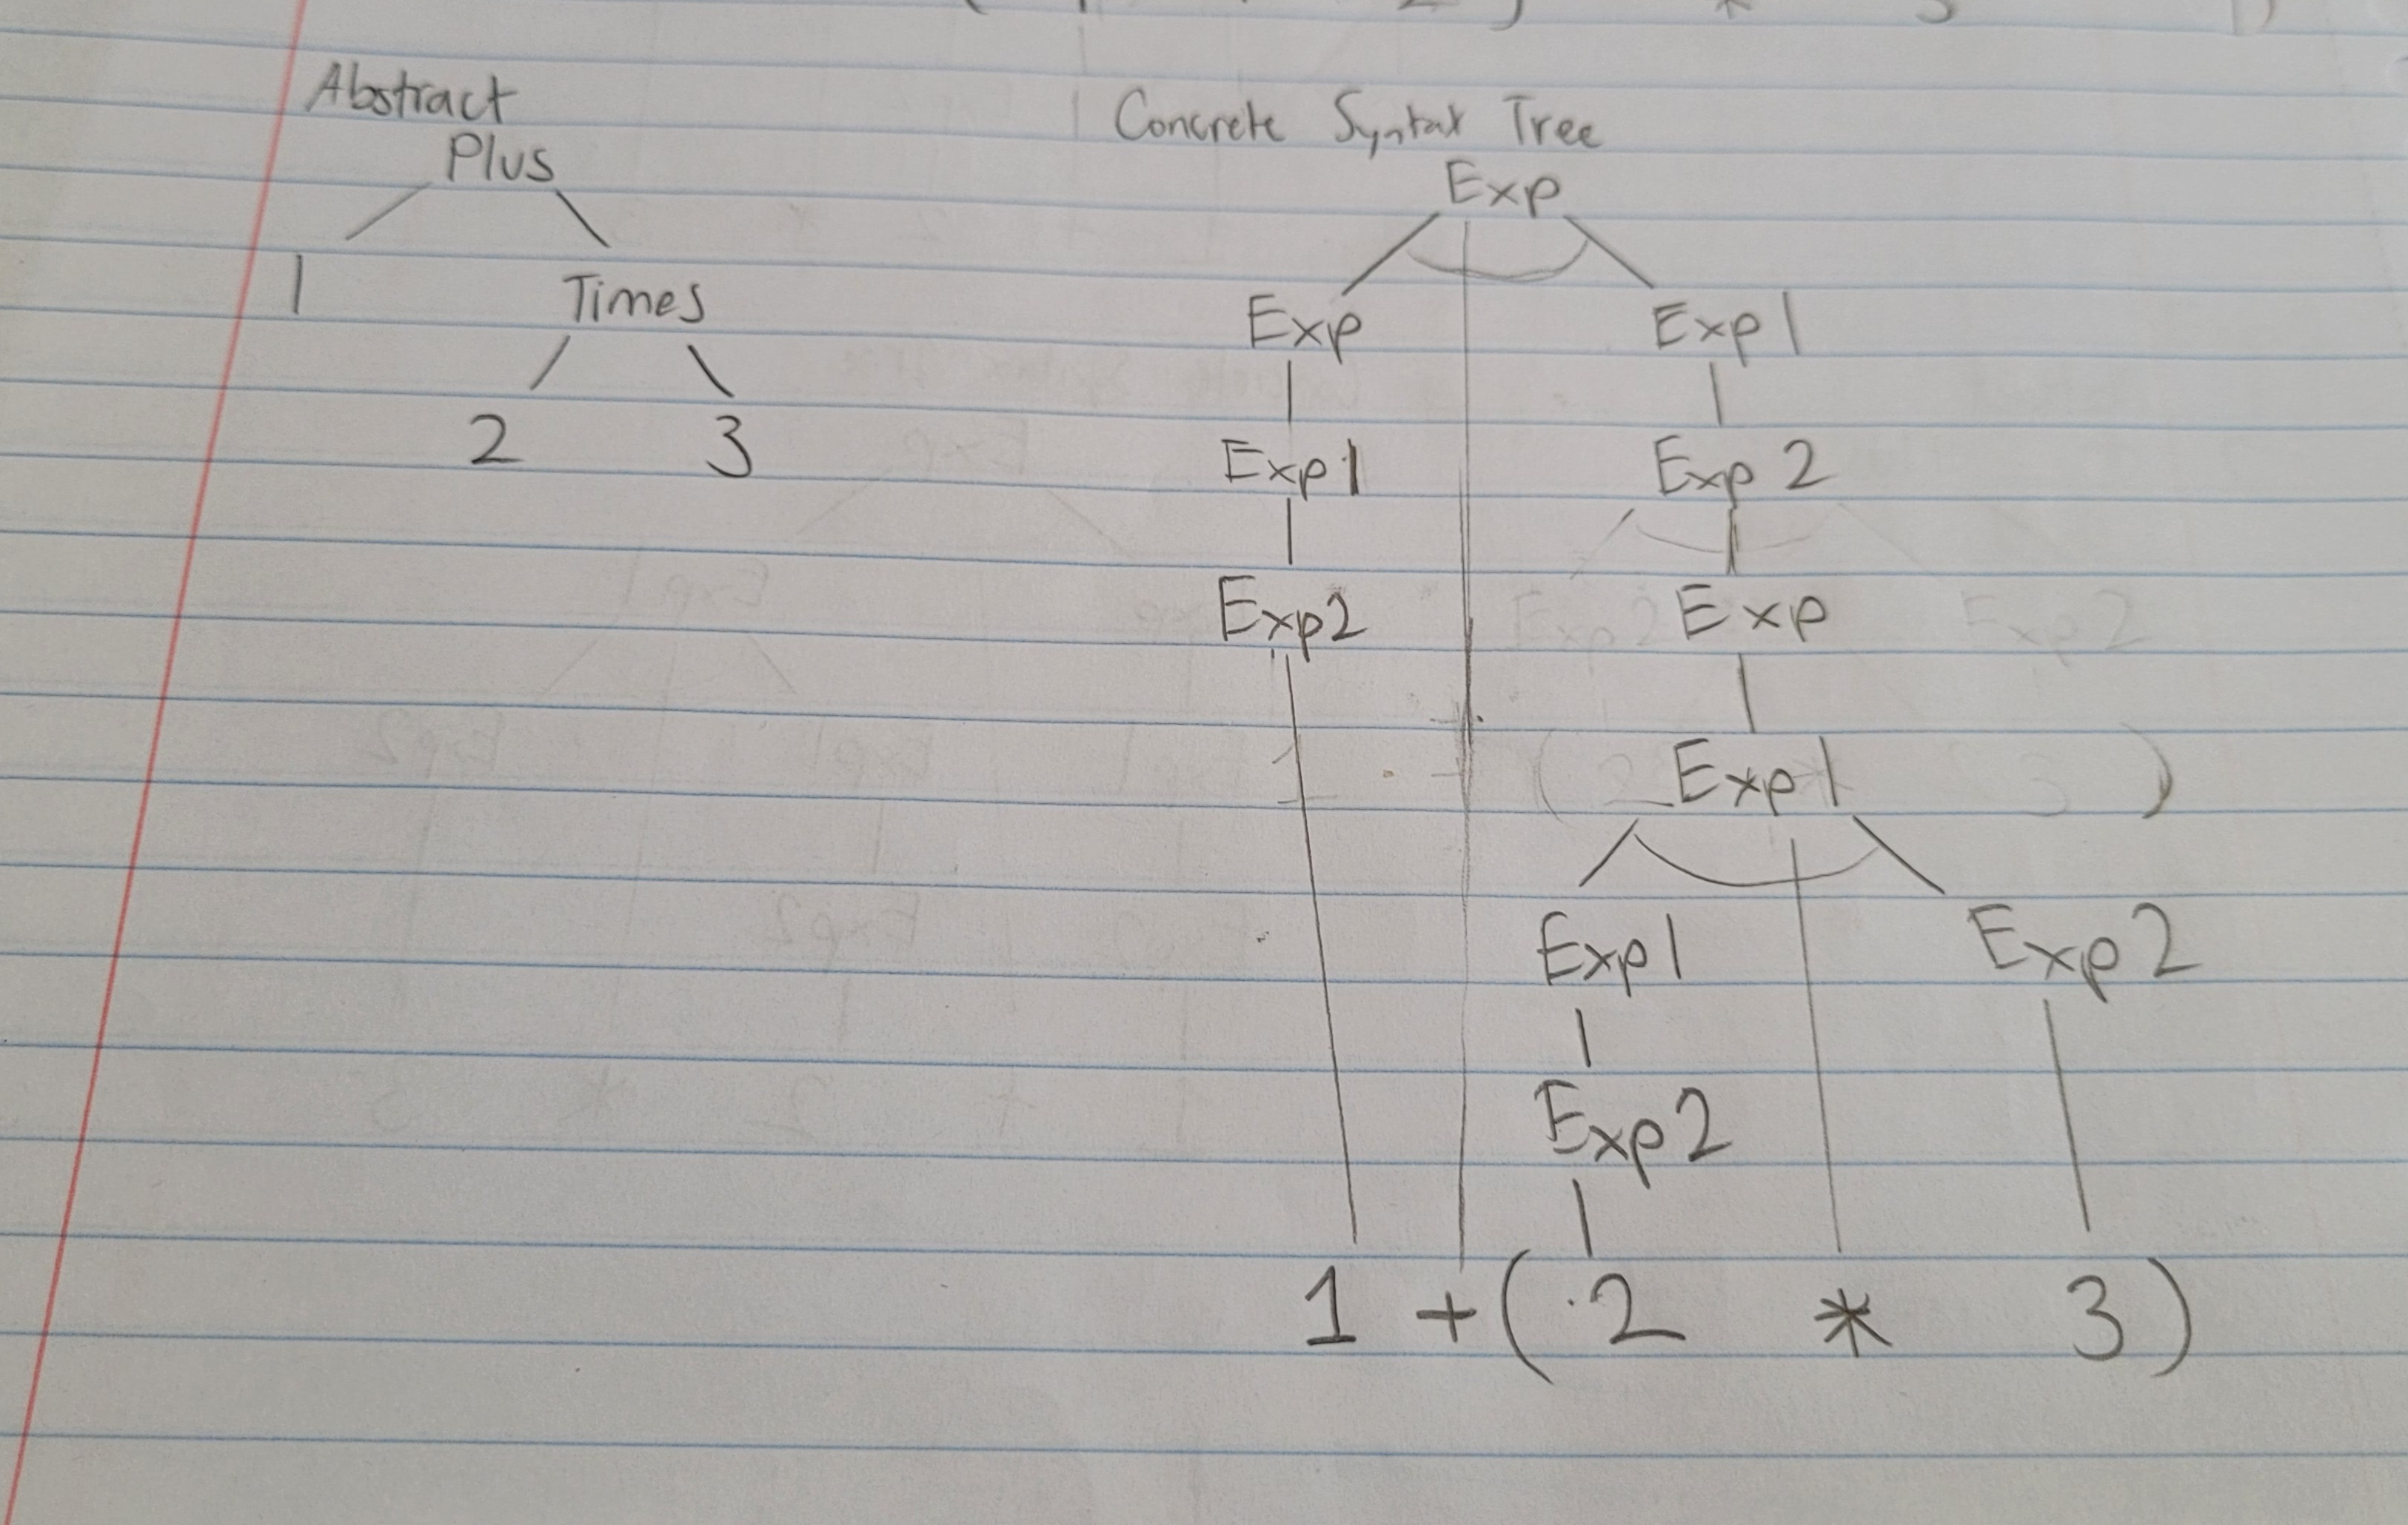
\includegraphics[width=15cm, height=8cm]{Report Images/week4_3.jpg}
\begin{lstlisting}
Plus (Num 1) (Times (Num 2) (Num 3))
\end{lstlisting}

The Abstract Syntax Tree of $(1 + 2) * 3$ is:

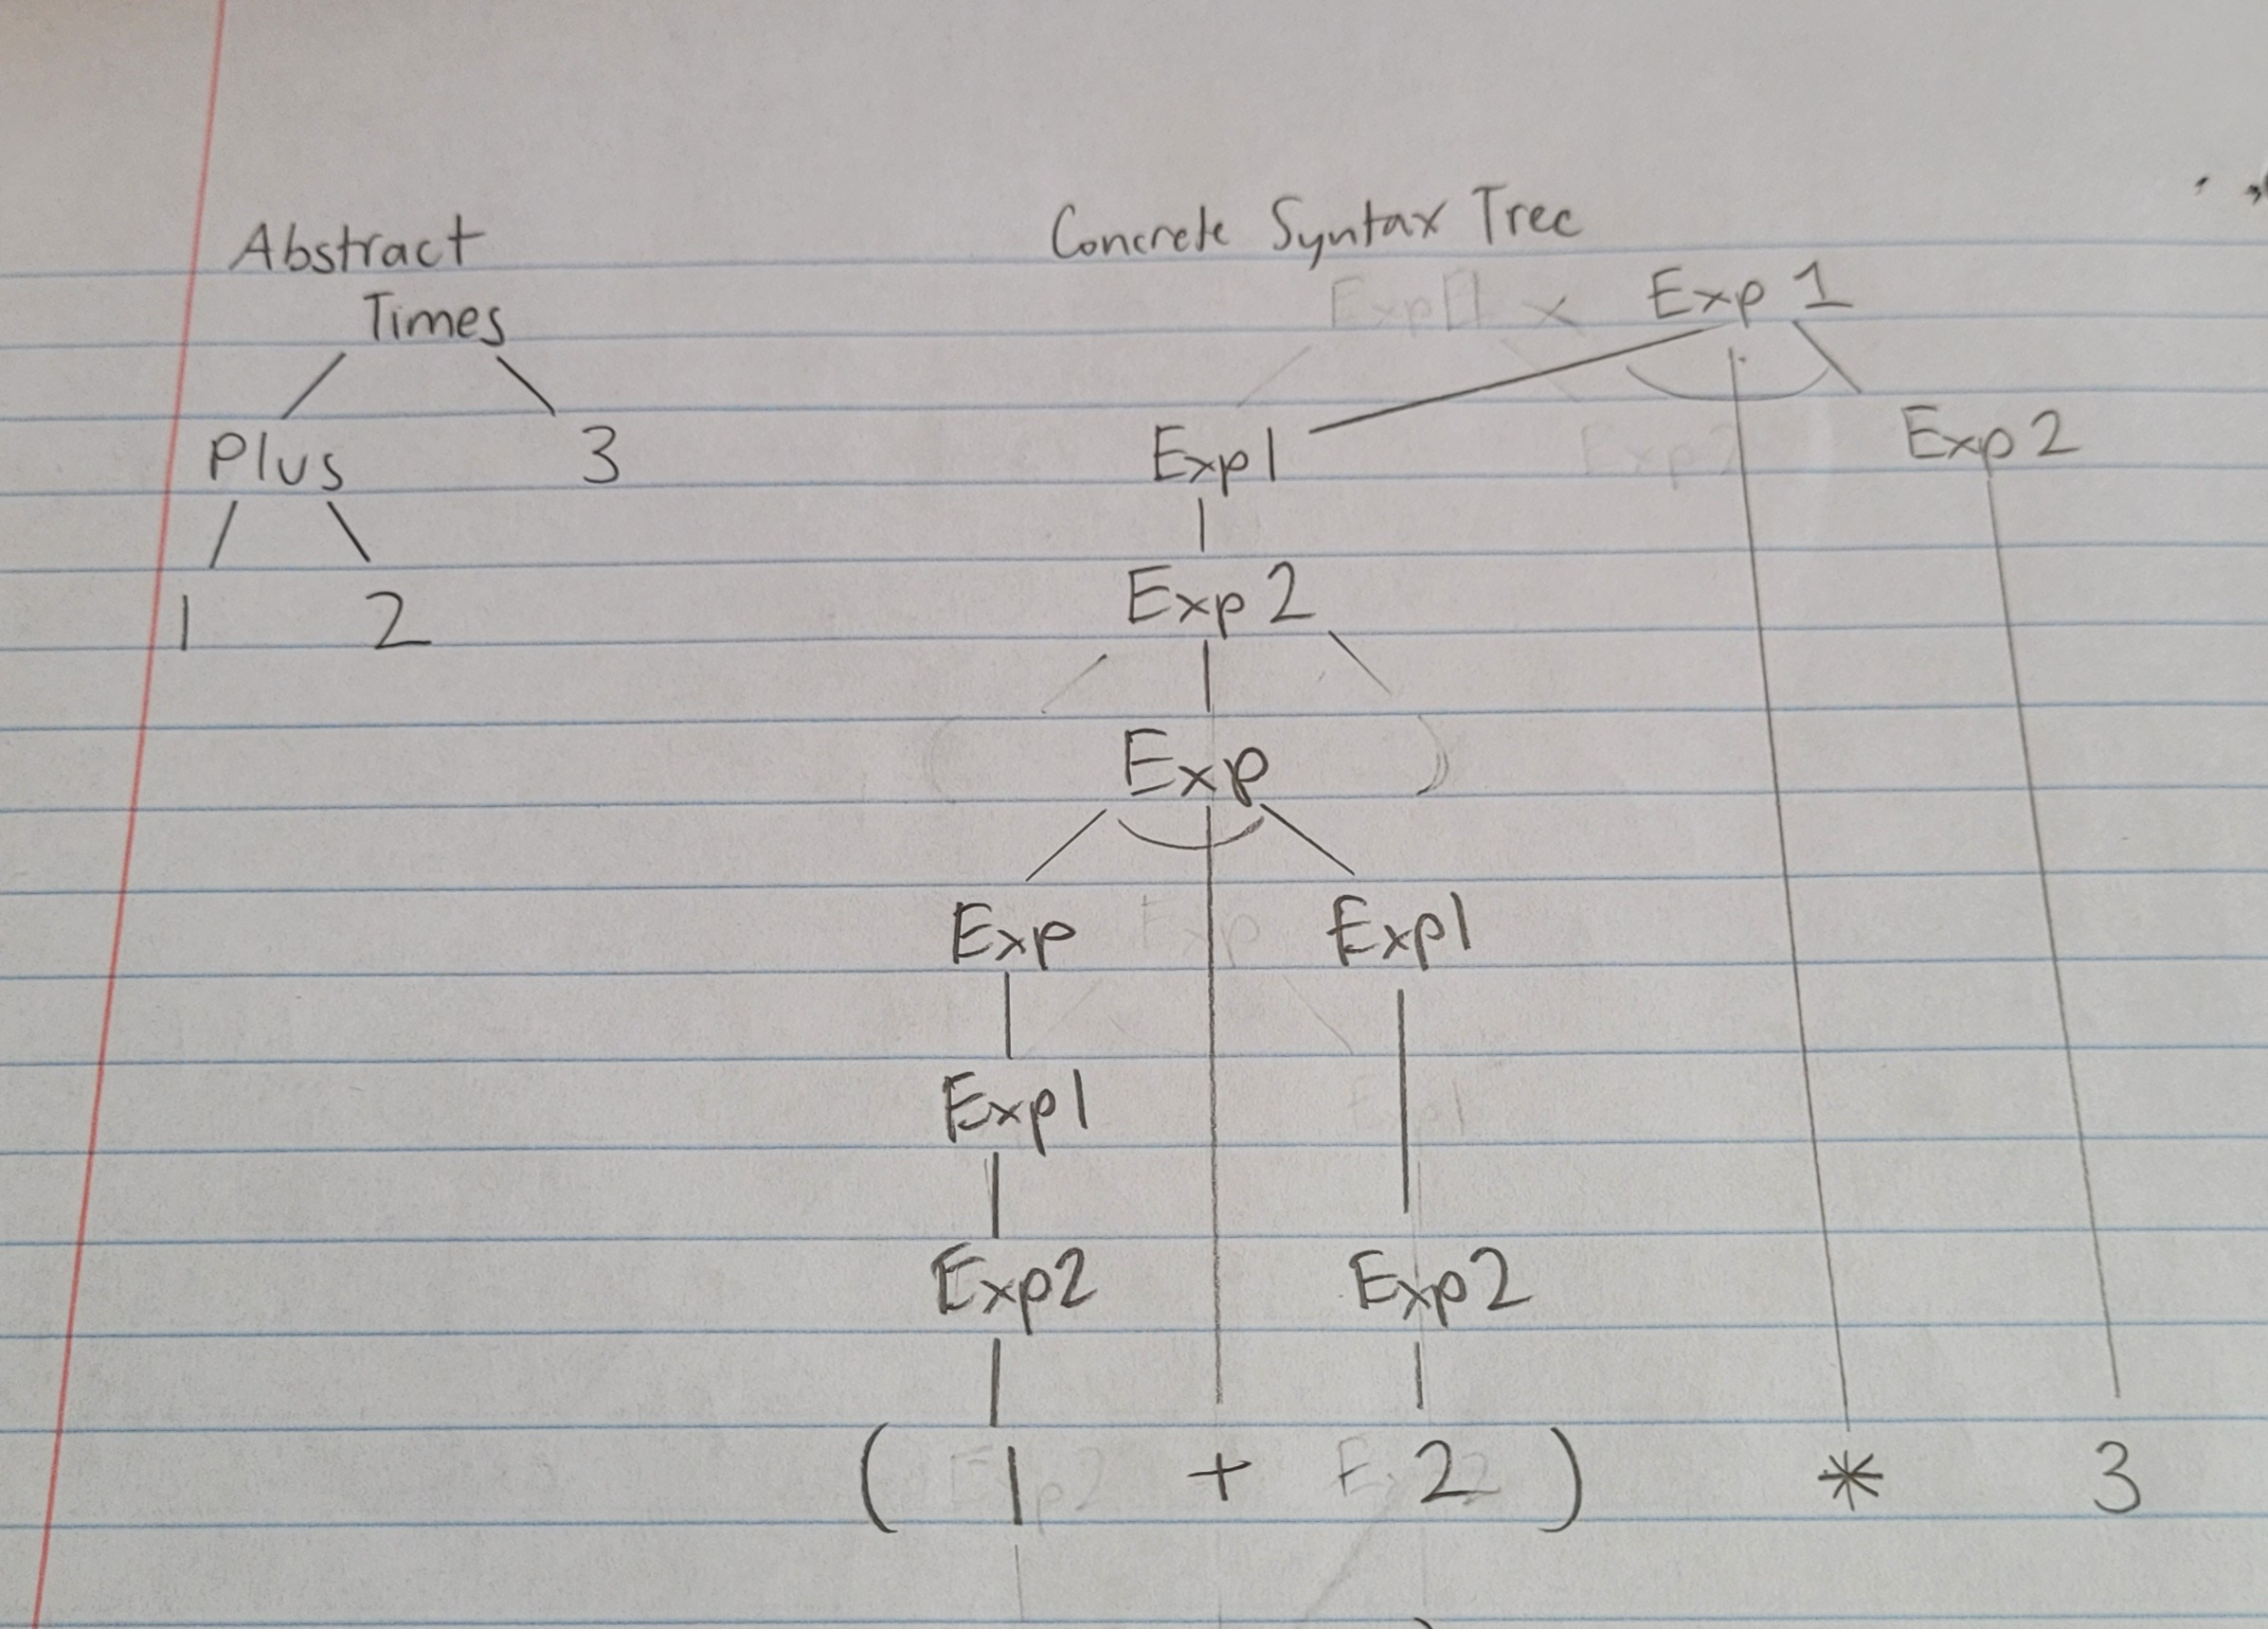
\includegraphics[width=15cm, height=8cm]{Report Images/week4_4.jpg}
\begin{lstlisting}
Times (Plus (Num 1) (Num 2)) (Num 3)
\end{lstlisting}

The Abstract Syntax Tree of $1 + 2 * 3 + 4 * 5 + 6$ is:

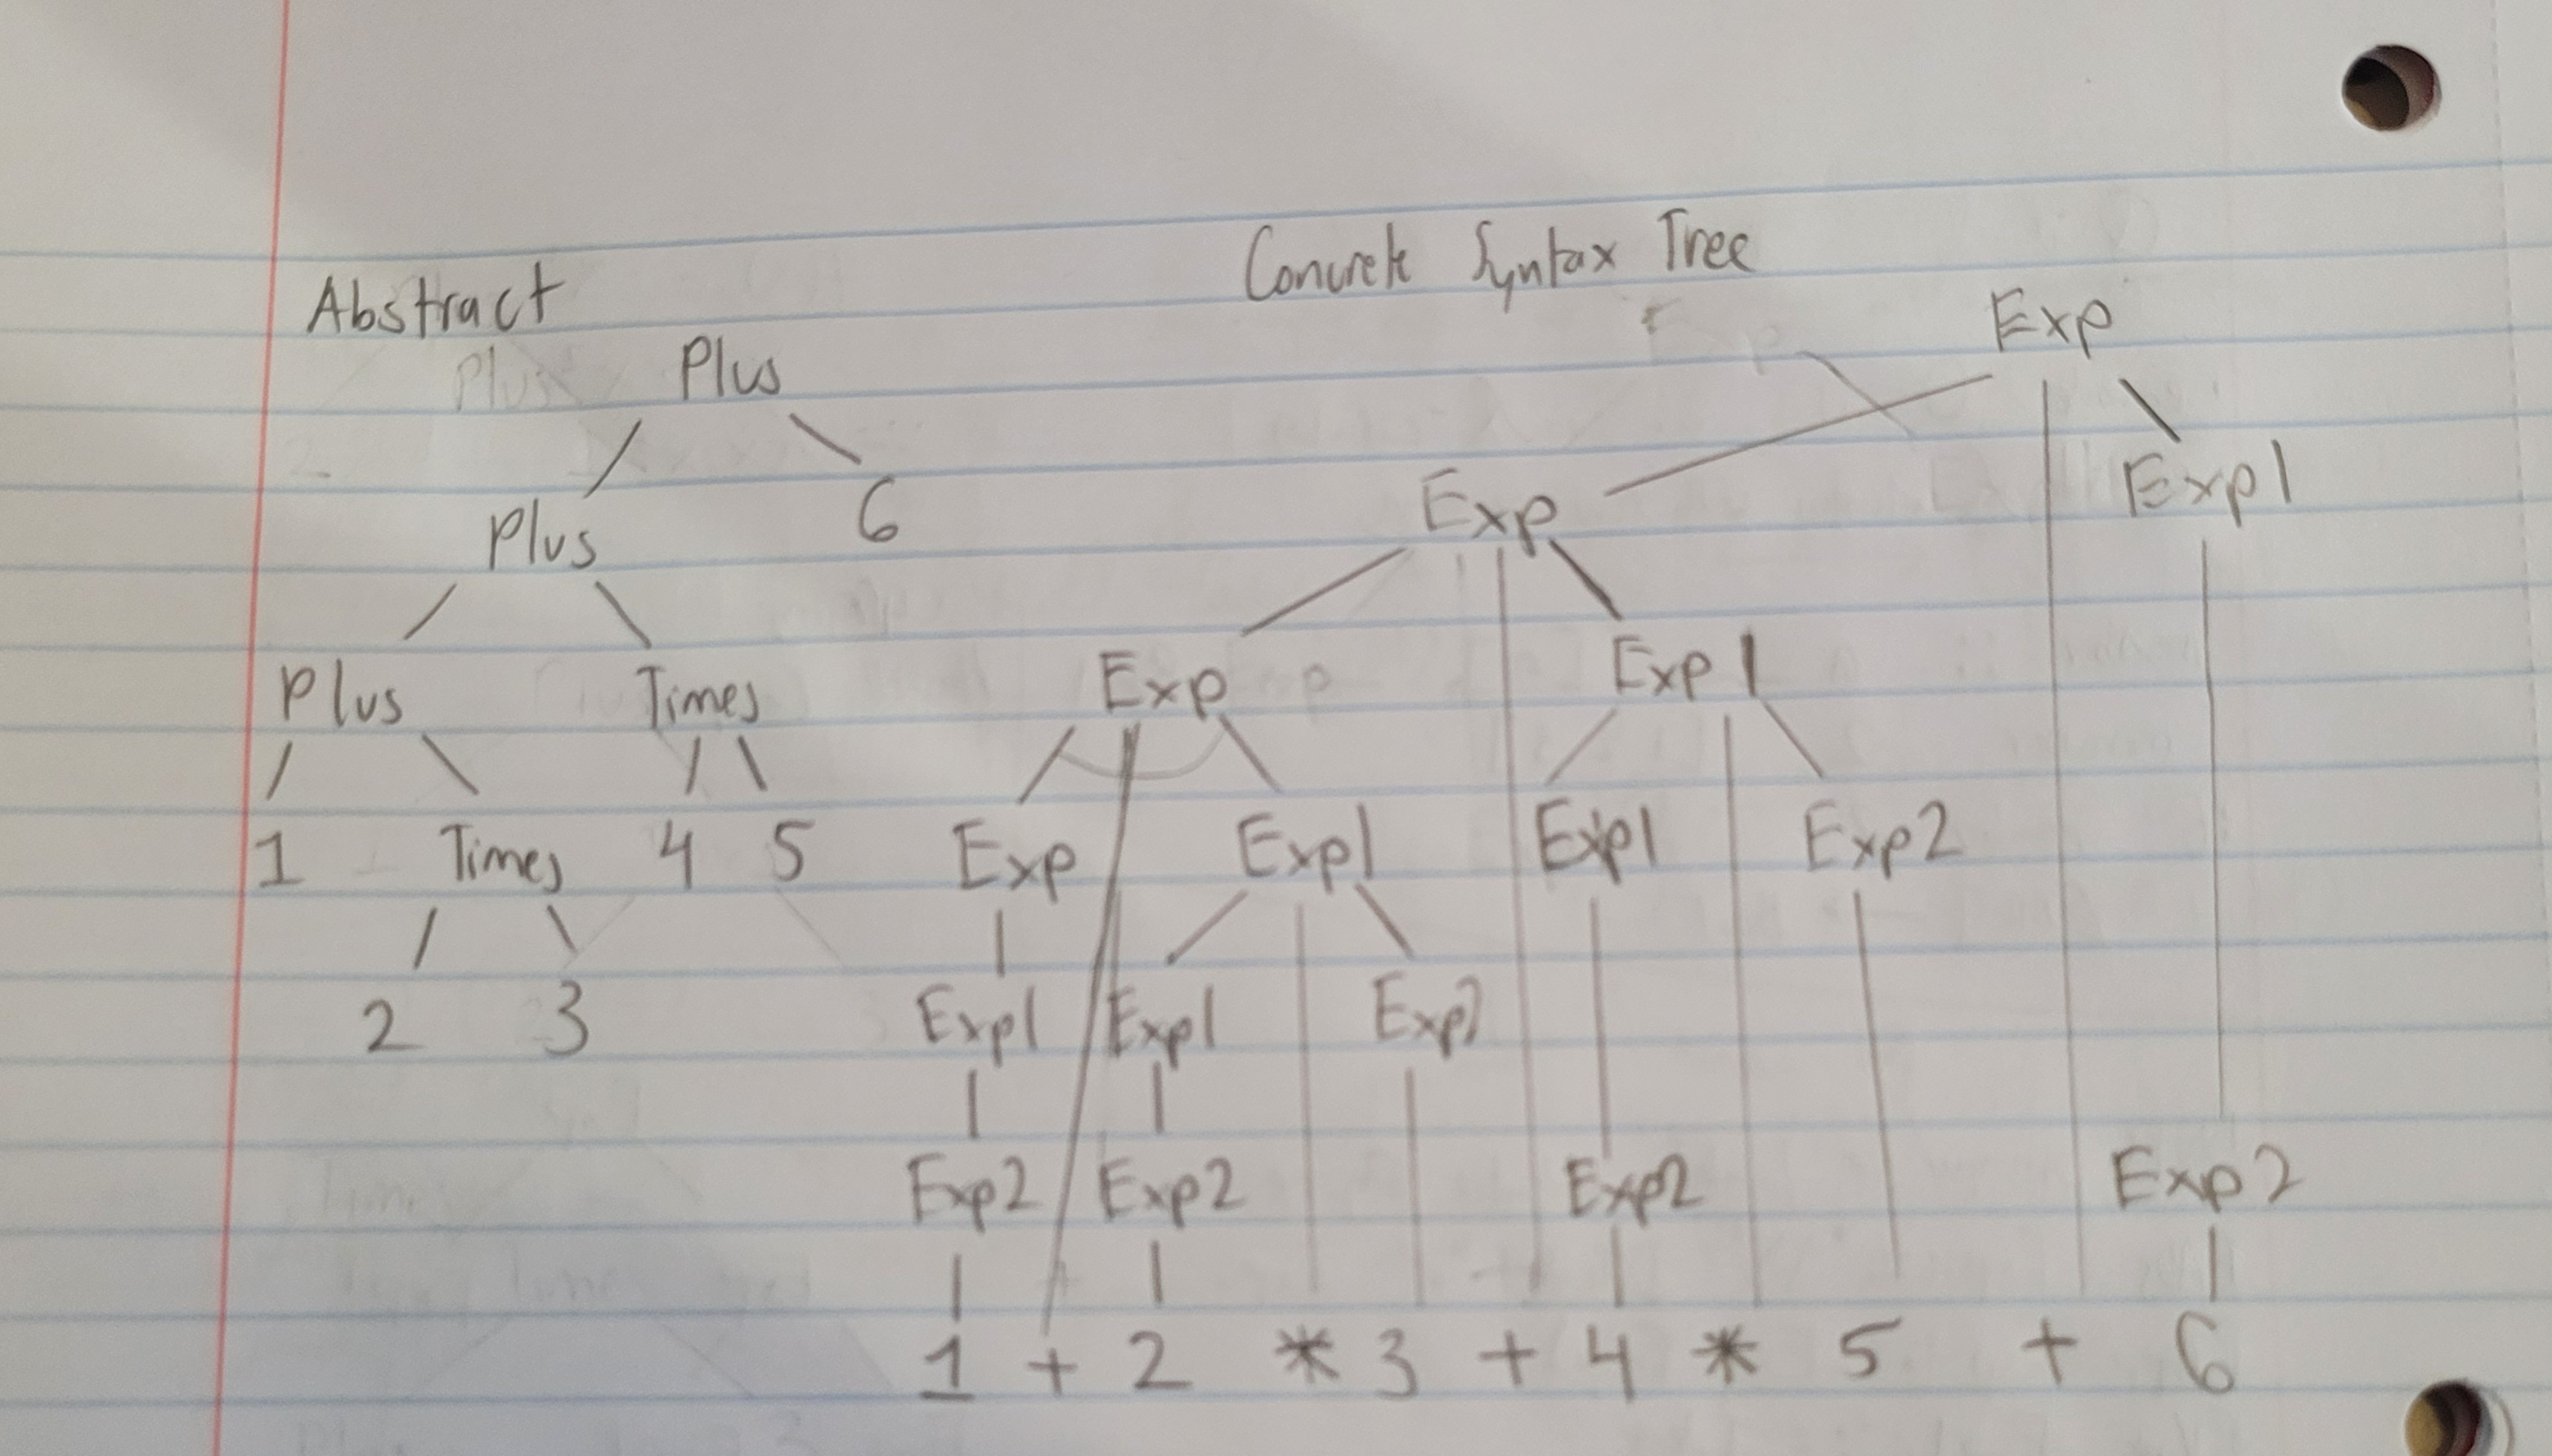
\includegraphics[width=15cm, height=8cm]{Report Images/week4_5.jpg}
\begin{lstlisting}
Plus (Plus (Plus (Num 1) (Times (Num 2) (Num 3))) (Times (Num 4) (Num 5))) (Num 6)
\end{lstlisting}


The abstract syntax tree of $1+2+3$ would be identical to the one of $(1+2)+3$ as the compiler would calculate from left to right as there are no other higher-order operations aside from addition.
\end{document}
